\section*{\centering Elliptisk satellitbana}

\subsection*{Teori}
Detta avsnitt grundar sig på kapitel 33 i Tipler och Moscas bok \textit{Physics for Scientists and Engineers} (2008).
\vspace{5mm}

Enligt Keplers andra lag är hastigheten för en planet, som färdas i en ellips runt solen, sådan att en radie från solen till planeten alltid sveper över en lika stor area på samma tid.

Om en satellit färdas i en elliptisk bana runt jorden så är arean $dA$ som radien $\Vec{r}$ från jorden till satelliten sveper över en tid $dt$ hälften av arean i det parallellogram som bildas av radien och satellitens färdsträcka $\Vec{v}dt$.

\begin{equation}
    dA = \dfrac{1}{2} \left|\Vec{r}\Vec{v}dt \right| =\dfrac{\left|\Vec{r}m\Vec{v} \right|}{2m}dt 
\end{equation}

Eftersom att satelliten rör sig i en fix bana så förändras inte dess totala mekaniska energi, vilket innebär att rörelsemängdsmomentets storlek $\left|\Vec{r}m\Vec{v} \right|$ är konstant. Detta betyder i sin tur att även $rv\text{sin}(\phi)$, där $\phi$ är vinkeln mellan hastighetsvektorn (som kan påpekas är i linje med tangenten till den elliptiska banan i den punkt där satelliten befinner sig) och radien, är konstant. Eftersom $\phi$ är 90 grader både i perigeum (punkten i rörelsebanan där radien är kortast) och apogeum (motsatsen till perigeum) så är

\begin{equation}
    v_a r_a = v_p r_p.
\end{equation}


\subsection*{Resultat \& beräkningar}
$r_p =  8.37\cdot10^{6}$ m \\
$r_a =  25.1\cdot10^{6}$ m \\
$v_p =  8450$ m/s \\
$v_a r_a = v_p r_p \implies v_a = \dfrac{r_p}{r_a}v_{p}$ \\   
$v_a = 2800$ m/s \\
Satellitens minsta hastighet är 2800 m/s.

\begin{figure}[H]
    \centering
    \captionsetup{justification=centering,margin=2cm}
    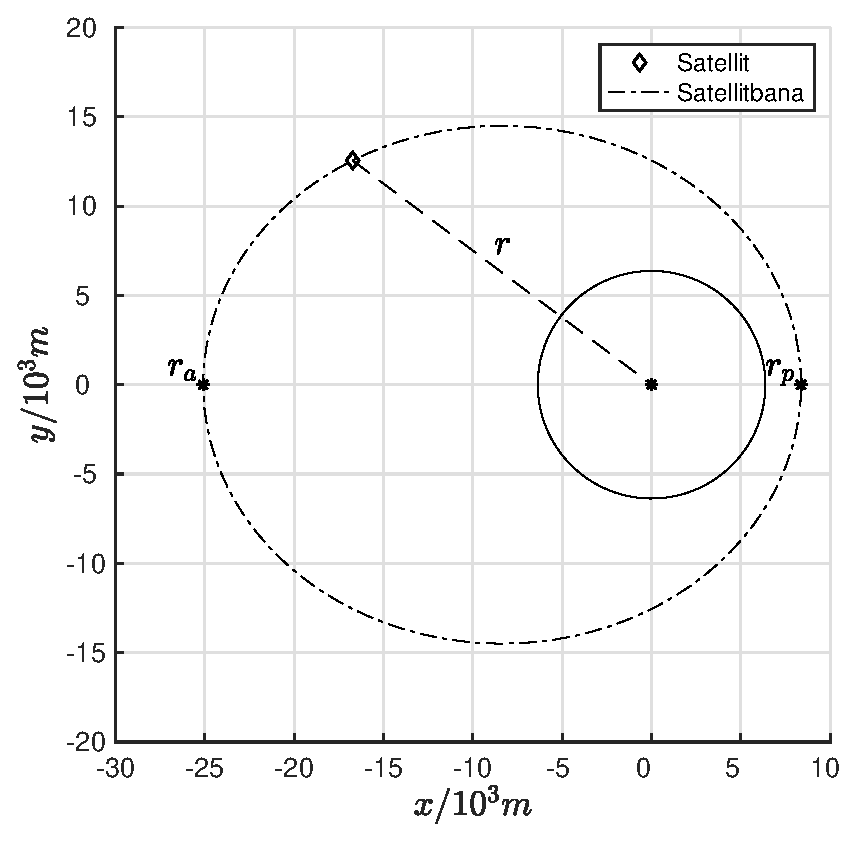
\includegraphics[scale=0.7]{Resources/Graphics/fig3_1.eps}
    \caption{Illustration av satellitens omloppsbana kring jorden.}
    \label{fig:3_1}
\end{figure}

\subsection*{Kommentar}
Den minsta hastigheten för satelliten äger rum i apogeum. Detta förklaras av Keplers andra lag som säger att radien alltid sveper över samma area under samma tid. Eftersom satelliten befinner sig längst bort i apogeum så måste därför hastigheten vara mindre i denna punkt än i resten av den elliptiska rörelsebanan.

\subsection*{Referenser}
Mosca, Gene; Tipler, A., Paul. 2008. \textit{Physics for Scientists and Engineers}. 6:e upplagan. W.H. Freeman and Company, New York.

\np
\subsection*{MatLab-kod}
\lstinputlisting[caption={\quad},firstline=3] {Resources/Code/3.m}